\documentclass[12pt]{article}

\newcommand{\CiteMathPackage}{../../math}
\newcommand{\CiteReference}{../reference.bib}

% Packages
\usepackage{setspace,geometry,fancyvrb,rotating}
\usepackage{marginnote,datetime,enumitem}
\usepackage{titlesec,indentfirst}
\usepackage{amsmath,amsfonts,amssymb,amsthm,mathtools}
\usepackage{threeparttable,booktabs,adjustbox}
\usepackage{graphicx,epstopdf,float,soul,subfig}
\usepackage[toc,page]{appendix}
\usdate

% Page Setup
\geometry{scale=0.8}
\titleformat{\paragraph}[runin]{\itshape}{}{}{}[.]
\titlelabel{\thetitle.\;}
\setlength{\parindent}{10pt}
\setlength{\parskip}{10pt}
% \usepackage{fourier}    		  % Favourite Font
\usepackage{Alegreya}
\usepackage[T1]{fontenc}

%% Bibliography
\usepackage{natbib,fancybox,url,xcolor}
\definecolor{MyBlue}{rgb}{0,0.2,0.6}
\definecolor{MyRed}{rgb}{0.4,0,0.1}
\definecolor{MyGreen}{rgb}{0,0.4,0}
\definecolor{MyPink}{HTML}{E50379}
\definecolor{MyOrange}{HTML}{FF5733}
\newcommand{\highlightR}[1]{{\emph{\color{MyRed}{#1}}}} 
\newcommand{\highlightB}[1]{{\emph{\color{MyBlue}{#1}}}}
\newcommand{\highlightP}[1]{{\emph{\color{MyPink}{#1}}}}
\newcommand{\highlightO}[1]{{\emph{\color{MyOrange}{#1}}}}
\usepackage[bookmarks=true,bookmarksnumbered=true,colorlinks=true,linkcolor=MyBlue,citecolor=MyRed,filecolor=MyBlue,urlcolor=MyGreen]{hyperref}
\bibliographystyle{econ}

%% Theorem Environment
\theoremstyle{definition}
\newtheorem{assumption}{Assumption}
\newtheorem{definition}{Definition}
\newtheorem{theorem}{Theorem}
\newtheorem{proposition}{Proposition}
\newtheorem{lemma}[theorem]{Lemma}
\newtheorem{example}{Example}
\newtheorem{corollary}[theorem]{Corollary}
\usepackage{mathtools}
\usepackage{\CiteMathPackage}

\begin{document}

%??%??%??%??%??%??%??%??%??%??%??%??%??%??%??%??%??%??%??%??%??%??
%?? title
%??%??%??%??%??%??%??%??%??%??%??%??%??%??%??%??%??%??%??%??%??%??

\title{\bf Offshoring and Occupational Specificity of Human Capital, Review of Economic Dynamics, 2014}
\author{Wenzhi Wang \thanks{This note is written in my pre-doc period at the University of Chicago Booth School of Business.} } 
\date{\today}
\maketitle

\citet{ritterOffshoringOccupationalSpecificity2014}

\setcounter{section}{2}

\section{Model}

\subsection{Environment}

The economy is populated by a measure one of infinitely lived workers. Workers' preferences are linear in consumption and they discount the future at rate $\b \in \bp{0,1}$. Time is discrete and indexed by $t = 0, 1, 2, \ldots$.

\subsubsection{Production}

A non-tradable final consumption good $Y$ is produced competitively using $N$ distinct intermediate inputs, called tasks:
\begin{equation}
    \notag 
    Y = \bs{\sum_{i=1}^{N} y_i^{\rho}}^{\frac{1}{\rho}},
\end{equation}
where $\rho < 1$ governs the elasticity of substitution between tasks. 

For each task, there is a large number of producers. Labor is the only variable input in production; there is also a fixed factor for each task, to which each agent holds an equal share. The fixed factor is implied by the decreasing returns technology, which assures the task has a positive mass of workers, even in the presence of international competition. The representative task producer's technology is given by:
\begin{equation}
    \notag 
    y_i\of{z, l} = z_i l_i^\a, \a < 1,
\end{equation}
where $z_i$ is a time-invariant task-specific productivity parameter and $l_i$ is the total effective labor employed in producing task $i$. 

A subset $M < N$ of the tasks are tradable; the economy is small relative to the rest of the world and so it takes the world market price as given. There are no trade costs, the domestic price for tradable tasks equals their world market price, $p_i = p_i^w$. 

Perfect competition in the production of the final good implies that the price index for the final good is given by 
\begin{equation}
    \label{1}
    P=\left(\sum_{i=1}^N p_i^{\frac{-\rho}{1-\rho}}\right)^{\frac{\rho-1}{\rho}}
\end{equation}
and the resulting demand for each task is given by 
\begin{equation}
    \label{2}
    y_i^d=\left(\frac{P}{p_i}\right)^{\frac{1}{1-\rho}} Y
\end{equation}

\subsubsection{Labor Market}

The labor market consists of many occupations where each occupation fulfills exactly one task. While there are search frictions between occupations, the labor market within an occupation is competitive, so the real wage per effective unit of labor is the value of its marginal product:
\begin{equation}
    \label{3}
    w_i = p_i \a z_i l_i^{\a - 1}.
\end{equation}
Workers are either employed in an occupation or are unemployed. At the beginning of the period, unemployed workers search for employment by applying to an occupation, i.e., search is directed. After applying, with probability $\f$ the unemployed worker gets matched with the occupation to which she applied and draws her permanent worker-occupation specific productivity $s$ from some distribution $F\of{s}$. With probability $1 - \f$, she remains unemployed and receives a payoff $b$ from home production. 

Workers can become unemployed by quitting or by exogenously separating. At the beginning of each period, an employed worker decides whether to remain in the current occupation and retain the current productivity draw $s$, or become unemployed and search for a new line of work. At the end of each period (except the first period in the occupation), a worker may become separated from the occupation exogenously at rate $\d^j$, where the superscript $j$ indicates that the separation rate depends on the worker's human capital level. Workers who separate from their occupation may begin applying to a new one immediately. The timing assumptions imply that a worker will remain in an occupation for at least one period. 

\begin{figure}[H]
    \noindent\caption{Total fertility rate in each year}
    \begin{center}
        \resizebox{0.7\textwidth}{!}{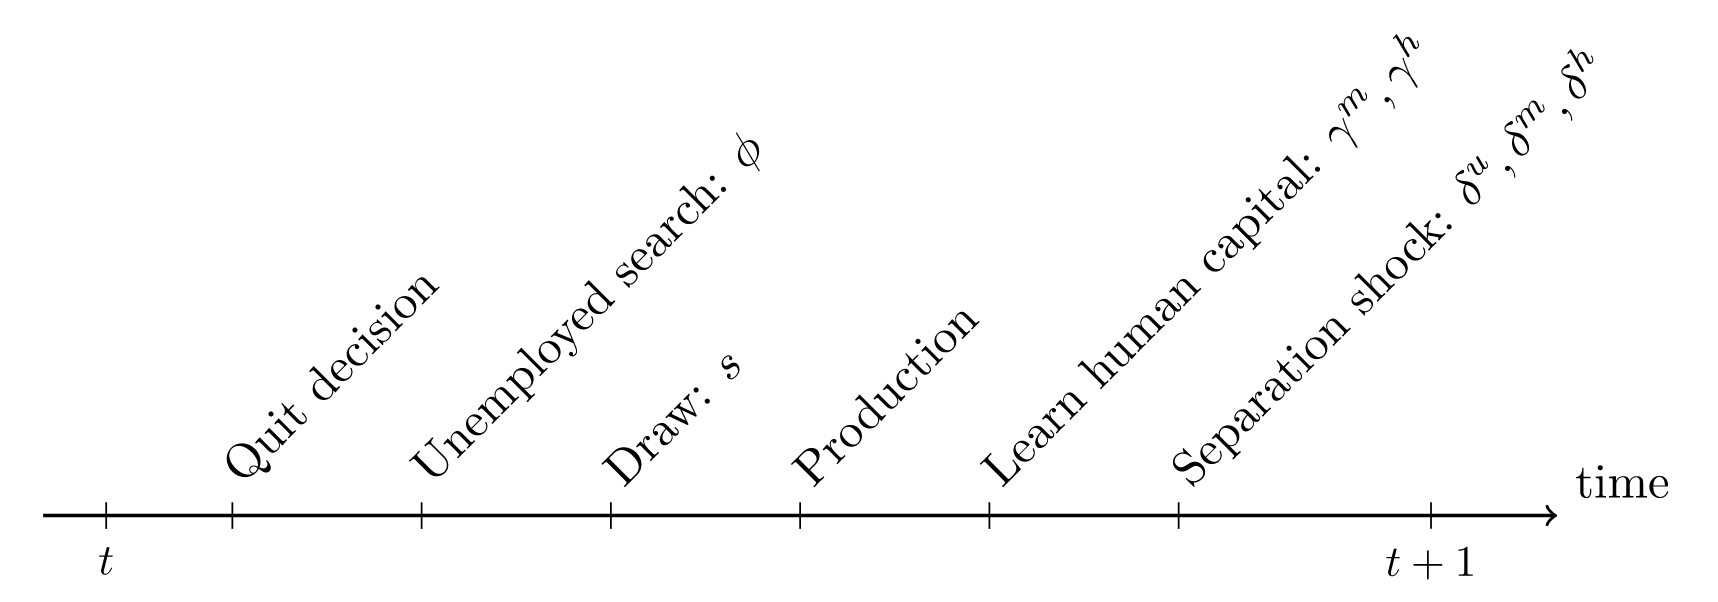
\includegraphics{ritterOffshoringOccupationalSpecificity2014_fig2.png}}
        \label{ritterOffshoringOccupationalSpecificity2014_fig2}
    \end{center}
\end{figure}

\subsubsection{Human Capital}

Human capital is occupation specific and is accumulated through learning-by-doing. There are three levels of occupation-specific skills. A worker enters the occupation as an unskilled worker and, at the end of each period (except the first one), the worker may acquire the specific human capital necessary to become a medium skilled worker. The arrival rate of the skill shock for an unskilled worker is $\g^m$. Similarly, a medium worker becomes high-skilled at rate $\g^h$.

The increase in productivity upon becoming skilled varies between occupations, but within an occupation all agents experience the same relative increase in their productivity. While an unskilled worker has $s$ units of productive time each period, a medium skilled worker has $a_i^m$s and a high skilled worker has $a_i^h$s, with $1 < a_i^m < a_i^h$. After becoming skilled, a worker remains skilled until she leaves the occupation. The time line is depicted in Figure \ref{ritterOffshoringOccupationalSpecificity2014_fig2}.

\subsection{The Worker's Problem}

\subsubsection{Employed Worker}

A worker employed in occupation $i$ at the beginning of each period faces the decision whether to quit and search for a new line of work or remain employed in the current occupation. Let $\mu$ denote the distribution of workers across occupations, idiosyncratic productivities, and occupation specific human capital at the beginning of a period and $U\of{\mu}$ the associated value of searching. Then the Bellman equation for a high skilled worker with productivity $s$ in occupation $i$ is given by:
\begin{equation}
    \label{4}
    V_i^h\of{s, \mu} = \max\bc{J_i^h\of{s, \mu}; U\of{\mu}},\quad \text{ with }
\end{equation}
\begin{equation}
    \label{5}
    J_i^h\of{s, \mu} = s a_i^h w_i + \b \bs{\bp{1 - \d^h} V_i^h\of{s, \mu^\prime} + \d^h U\of{\mu^{\prime}}}.
\end{equation}
Similarly, the Bellman equations for medium and unskilled workers are given by:
\begin{equation}
    \label{6}
    V_i^m\of{s, u} = \max\bc{J_i^m\of{s, \mu}; U\of{\mu}},\quad \text{ with }
\end{equation}
\begin{equation}
    \label{7}
    J_i^m\of{s, \mu} = s a_i^m w_i + \b \bc{\bp{1 - \d^m} \bs{\g^hV_i^h\of{s, \mu^\prime} + \bp{1-\g^h} V_i^m\of{s, \mu^{\prime}}} + \d^m U\of{\mu^{\prime}}}, \quad \text{ and }
\end{equation}
\begin{equation}
    \label{8}
    V_i^u\of{s, u} = \max\bc{J_i^u\of{s, \mu}; U\of{\mu}},\quad \text{ with }
\end{equation}
\begin{equation}
    \label{9}
    J_i^u\of{s, \mu} = s w_i + \b \bc{\bp{1 - \d^u} \bs{\g^mV_i^m\of{s, \mu^\prime} + \bp{1-\g^m} V_i^u\of{s, \mu^{\prime}}} + \d^u U\of{\mu^{\prime}}},
\end{equation}
respectively. Each worker takes the value of search, $U$, and the future values of $V^u, V^m$, and $v^h$ as given. The values of staying in an occupation are increasing in the idiosyncratic productivity draw $s$. Therefore, the worker's optimal quitting decision can be described by a simple reservation productivity strategy: if the productivity draw exceeds the reservation level, the worker remains the in the occupation, otherwise the worker leaves and searches for a better match. Thus, a worker of type $j \in \bc{u, m, h}$ will leave occupation $i$ if 
\begin{equation}
    \label{10}
    J_i^j\of{s, \mu} < U\of{\mu} 
\end{equation}
and the optimal quitting policy can be described by an indicator function:
\begin{equation}
    \label{11}
    g_i^j(s, \mu)= \begin{cases}1 & \text { if }(\ref{10}) \text { holds, } \\ 0 & \text { otherwise. }\end{cases}
\end{equation}
In a stationary equilibrium in which the distribution of workers across occupations, productivities, and skills is time invariant and all prices and wages are constant, workers employed in each occupation will be either temporary or permanent. Temporary workers are those who entered at the beginning of the current period, received a low productivity draw, and will search again in the next period; permanent workers will remain and only leave after an exogenous separation. \footnote{An alternative way of modeling separations is to assume the workers receive a new occupation-specific productivity shock $s$ with probability $\xi$ every period. The probability of exiting an occupation in that case is $\xi F\of{\ol{s}_i^j}$, where $\ol{s}$ denotes the reservation productivity level. In steady state, this amounts to a constant separation rate that declines with the amount of human capital. }

\subsubsection{Unemployed Worker}

An unemployed worker who is currently searching applies to the occupation that offers the highest expected value of applying. Hence, the Bellman equation for unemployed workers is given by:
\begin{equation}
    \label{12}
    U\of{\mu} = \max_{i \in N} \bc{\f \E_s\bs{J_i^1\of{s, \mu}} + \bp{1-\f} \bs{b + \b U\of{\mu^{\prime}}}},
\end{equation}
where $\E_s$ denotes the expectation operator over the possible idiosyncratic productivities $s$ and $J_i^1\of{s, \mu}$ denotes the value of entering th occupation $i$ with draw $s$, 
\begin{equation}
    \label{13}
    J_i^1 = sw_i + \b V_i^u\of{s, \mu^{\prime}}.
\end{equation}
This takes into account that a worker who just entered the occupation may not acquire specific human capital and is not subject to exogenous separation at the end of the last period. 

Search is directed, so any occupation that wishes to attract applicants must offer the same expected value as other occupations. If the value of applying to occupation $i$ is less than for other occupations, no worker will apply and employment in that occupation will shrink due to the exogenous separation and quitting. As is common in the directed search literature, I focus on the symmetric mixed-strategy equilibrium in which identical workers use identical, mixed application strategies. 

\subsubsection{Employment Dynamics}

During the production stage, workers are either employed or unemployed. Employed workers vary by idiosyncratic productivity and their specific human capital. Between two production stages, workers may endogenously or exogenously leave an occupation and may acquire human capital. Let $g^A\of{\mu} = \bp{g_1^A\of{\mu}, \ldots, g_N^A\of{\mu}}$ denote the policy function describing the optimal mixed application strategy for workers and $A\of{\mu}$ the total number of applicants. Thus, the total number of workers applying to occupation $i$ is $A_i\of{\mu} = g_i^A\of{\mu} A\of{\mu}$.

The resulting law of motion for the beginning of the period distribution of workers is given by 
\begin{equation}
    \label{14}
    \mu_i^{h^{\prime}}=\left(1-\delta^h\right)\left(g^h(s, \mu) \mu_i^h+\gamma^h g^m(s, \mu) \mu_i^m\right),
\end{equation}
\begin{equation}
    \label{15}
    \mu_i^{m^{\prime}}=\left(1-\delta^m\right)\left(g^m(s, \mu)\left(1-\gamma^h\right) \mu_i^m+\gamma^m g^u(s, \mu) \mu_i^u\right),
\end{equation}
\begin{equation}
    \label{16}
    \mu_i^{u^{\prime}}=\left(1-\delta^u\right)\left(1-\gamma^m\right) g^u(s, \mu) \mu_i^u+\phi A_i(\mu) d F(s).
\end{equation}

\subsection{Equilibrium}

A competitive equilibrium for given world prices $\bc{p_i^2}_{i \in M}$ consists of 
\begin{itemize}[topsep=0pt, leftmargin=20pt, itemsep=0pt]
	\setlength{\parskip}{10pt} 
	\item value functions for workers $\bc{V_i^j\of{s, \mu}, J_i^j\of{s, \mu}, J_i^1\of{s, \mu}}_{i \in N, j \in \bc{u, m, h}}$,
	\item associated policy functions $\bc{g_i^j\of{s, \mu}, g_i^A\of{\mu}}_{i \in N, j \in \bc{u, m, h}}$,
	\item the value of searching $U\of{\mu}$, 
	\item distribution of workers across occupations and skill levels $\mu$,
	\item domestic supply of and demand for intermediate tasks $\bc{y_i^S, y_i^D}_{i \in N}$ and final output $Y$,
	\item prices and wages $\bc{p_i, w_i}_{i \in N}$ for each task and an aggregate price index $P$,
\end{itemize}
such that:
\begin{enumerate}[topsep=0pt, leftmargin=20pt, itemsep=0pt, label=(\arabic*)]
	\setlength{\parskip}{10pt} 
	\item Given $U\of{\mu}$, prices, and wages, workers' value functions and associated policy functions maximize workers' individual utility. 
	\item The distribution of workers across sectors and skill levels follows (\ref{14})-(\ref{16}).
	\item Wages are determined competitively.
	\item The labor market in each occupation clears and aggregate feasibility is satisfied.
	\item The final good market and task markets clear.
	\item Trade is balanced: $0 = \sum_{i \in M} p_i^w \bp{y_i^S - y_i^D}$. 
\end{enumerate}


\section{Quantitative Analysis of US Trade Experience}

I calibrate the model to the US economy at the advent of the surge in service trade (1990) and then subject the economy to a trade shock that generates the magnitude of trade in goods adn services observed in 2010. \highlightO{In order to obtain the greatest possible short run effect, the full magnitude of the trade shock is assumed to hit the economy at once.} This is meant to capture a worst case scenario since it involves the most worker reallocation and hence the largest destruction of specific human capital. Assuming the claims that US workers are hurt by trade in high skill services are correct, this scenario would have to capture any such losses. In the long run, after reallocation and retraining, the gains from exploiting one's comparative advantage will dominate; the presumed losses stem from increased unemployment and the destruction of specific human capital in the short run. Were trade introduced very gradually, none or only a few skilled workers would switch occupations and minimal destruction of human capital would occur, which implies that there would be no short term distributional effects. In other words, losses resulting from the one-time shock presented in this section represent the upper bound on the potential short run cost of increased offshoring.

\subsection{Parametrization}

The model period is one year, as the focus of the analysis is the long-run transition from one steady state to another, rather than movements at a business cycle frequency. This is also consistent with the modeling choice of directed search. Consistent with the annual frequency, I set the discount factor at $\b = 0.96$. 

The parametrized economy consists of 500 distinct occupations. To restrict the number of human capital parameters that need to be calibrated, these occupations are grouped into five large occupation categories: \highlightO{tradable high/low psecific skill services, non-tradable high and low specific skill services, and tradable production occupations}. All occupations within a category differ with respect to their distinct type of specific human capital but are assumed to be identical with respect to their specific human capital acquisition processes and specific productivity distributions. In other words, each occupation is a separate island, occupations are only assumed to have similar levels of specific human capital. 

The parameters of the specific human capital process $\bp{a^m, a^h, \g^m, \g^h}$ are chosen to match the occupational tenure profile for occupations in each occupation category. The typical occupation-tenure profile is concave and levels off after about 10 years. I therefore set $a^m$ to match the average return to occupational-tenure profile within each category after 5 years and $a^h$ to match the return after 10 years; $\g^m$ and $\g^h$ are set such that a worker is expected to obtain the medium level after 5 and the high level of specific human capital after 10 years in the occupation. The probability of receiving an offer, $\f$, is set to generate an unemployment rate of 5.6\% and the value of home production, $b$, is set at a standard 60 percent replacement rate. 

The distribution of match-specific productivity shocks is assumed to be Pareto with a minimum of 1. The shape parameter of the distribution $\s$ can be set to match the fraction of workers in the first year of their occupational tenure. The probabilities of leaving an occupation after accumulating more than one year of tenure, $\d^j$, are chosen to match the hazard rate for workers with two to five years and more than five years of occupational tenure, respectively. 

Calibrating the parameters of the production process is less straightforward due to the lack of data available at the occupation level. For example, the labor share of output within an industry can easily be calculated from national accounts data, but there is no comparable information available for occupations, as the output of an occupation on its own is not easily measured. I therefore use the same curvature parameter of the task production function for all occupation groups and, as in \citet{kambourovOccupationalMobilityWage2009}, I set it to match an average labor share in the economy of 0.68. The productivity parameter for each task, $z_i$, is chosen such that all occupations have the same employment level in the initial 1990 steady state, with the productivity in non-tradable low skill services normalized to 1. The number of occupations in each category is then set such that each category's share of total employment matches that category's share in the 1990 census. \footnote{This approach is chosen over matching each of the 500 occupations' employment shares because it drastically reduces the number of parameters. For the quantitative exercise, the total number of workers exposed to trade and their initial level of human capital is crucial, not their occupation assignment.}

Finally, the elasticity of substitution between tasks, governed by $\rho$, is set to match the labor demand elasticity (elasticity of wages with respect to employment) at the 2-digit occupation level (22 groups) of 0.5, which implies $\rho = -1.5$. 






\bibliography{\CiteReference}


\end{document}
